
%% bare_conf.tex
%% V1.4b
%% 2015/08/26
%% by Michael Shell
%% See:
%% http://www.michaelshell.org/
%% for current contact information.
%%
%% This is a skeleton file demonstrating the use of IEEEtran.cls
%% (requires IEEEtran.cls version 1.8b or later) with an IEEE
%% conference paper.
%%
%% Support sites:
%% http://www.michaelshell.org/tex/ieeetran/
%% http://www.ctan.org/pkg/ieeetran
%% and
%% http://www.ieee.org/

%%*************************************************************************
%% Legal Notice:
%% This code is offered as-is without any warranty either expressed or
%% implied; without even the implied warranty of MERCHANTABILITY or
%% FITNESS FOR A PARTICULAR PURPOSE! 
%% User assumes all risk.
%% In no event shall the IEEE or any contributor to this code be liable for
%% any damages or losses, including, but not limited to, incidental,
%% consequential, or any other damages, resulting from the use or misuse
%% of any information contained here.
%%
%% All comments are the opinions of their respective authors and are not
%% necessarily endorsed by the IEEE.
%%
%% This work is distributed under the LaTeX Project Public License (LPPL)
%% ( http://www.latex-project.org/ ) version 1.3, and may be freely used,
%% distributed and modified. A copy of the LPPL, version 1.3, is included
%% in the base LaTeX documentation of all distributions of LaTeX released
%% 2003/12/01 or later.
%% Retain all contribution notices and credits.
%% ** Modified files should be clearly indicated as such, including  **
%% ** renaming them and changing author support contact information. **
%%*************************************************************************


% *** Authors should verify (and, if needed, correct) their LaTeX system  ***
% *** with the testflow diagnostic prior to trusting their LaTeX platform ***
% *** with production work. The IEEE's font choices and paper sizes can   ***
% *** trigger bugs that do not appear when using other class files.       ***                          ***
% The testflow support page is at:
% http://www.michaelshell.org/tex/testflow/



\documentclass[conference]{IEEEtran}
% Some Computer Society conferences also require the compsoc mode option,
% but others use the standard conference format.
%
% If IEEEtran.cls has not been installed into the LaTeX system files,
% manually specify the path to it like:
% \documentclass[conference]{../sty/IEEEtran}





% Some very useful LaTeX packages include:
% (uncomment the ones you want to load)


% *** MISC UTILITY PACKAGES ***
%
%\usepackage{ifpdf}
% Heiko Oberdiek's ifpdf.sty is very useful if you need conditional
% compilation based on whether the output is pdf or dvi.
% usage:
% \ifpdf
%   % pdf code
% \else
%   % dvi code
% \fi
% The latest version of ifpdf.sty can be obtained from:
% http://www.ctan.org/pkg/ifpdf
% Also, note that IEEEtran.cls V1.7 and later provides a builtin
% \ifCLASSINFOpdf conditional that works the same way.
% When switching from latex to pdflatex and vice-versa, the compiler may
% have to be run twice to clear warning/error messages.






% *** CITATION PACKAGES ***
%
%\usepackage{cite}
% cite.sty was written by Donald Arseneau
% V1.6 and later of IEEEtran pre-defines the format of the cite.sty package
% \cite{} output to follow that of the IEEE. Loading the cite package will
% result in citation numbers being automatically sorted and properly
% "compressed/ranged". e.g., [1], [9], [2], [7], [5], [6] without using
% cite.sty will become [1], [2], [5]--[7], [9] using cite.sty. cite.sty's
% \cite will automatically add leading space, if needed. Use cite.sty's
% noadjust option (cite.sty V3.8 and later) if you want to turn this off
% such as if a citation ever needs to be enclosed in parenthesis.
% cite.sty is already installed on most LaTeX systems. Be sure and use
% version 5.0 (2009-03-20) and later if using hyperref.sty.
% The latest version can be obtained at:
% http://www.ctan.org/pkg/cite
% The documentation is contained in the cite.sty file itself.






% *** GRAPHICS RELATED PACKAGES ***
%
\ifCLASSINFOpdf
  % \usepackage[pdftex]{graphicx}
  % declare the path(s) where your graphic files are
  % \graphicspath{{../pdf/}{../jpeg/}}
  % and their extensions so you won't have to specify these with
  % every instance of \includegraphics
  % \DeclareGraphicsExtensions{.pdf,.jpeg,.png}
\else
  % or other class option (dvipsone, dvipdf, if not using dvips). graphicx
  % will default to the driver specified in the system graphics.cfg if no
  % driver is specified.
  % \usepackage[dvips]{graphicx}
  % declare the path(s) where your graphic files are
  % \graphicspath{{../eps/}}
  % and their extensions so you won't have to specify these with
  % every instance of \includegraphics
  % \DeclareGraphicsExtensions{.eps}
\fi
% graphicx was written by David Carlisle and Sebastian Rahtz. It is
% required if you want graphics, photos, etc. graphicx.sty is already
% installed on most LaTeX systems. The latest version and documentation
% can be obtained at: 
% http://www.ctan.org/pkg/graphicx
% Another good source of documentation is "Using Imported Graphics in
% LaTeX2e" by Keith Reckdahl which can be found at:
% http://www.ctan.org/pkg/epslatex
%
% latex, and pdflatex in dvi mode, support graphics in encapsulated
% postscript (.eps) format. pdflatex in pdf mode supports graphics
% in .pdf, .jpeg, .png and .mps (metapost) formats. Users should ensure
% that all non-photo figures use a vector format (.eps, .pdf, .mps) and
% not a bitmapped formats (.jpeg, .png). The IEEE frowns on bitmapped formats
% which can result in "jaggedy"/blurry rendering of lines and letters as
% well as large increases in file sizes.
%
% You can find documentation about the pdfTeX application at:
% http://www.tug.org/applications/pdftex





% *** MATH PACKAGES ***
%
\usepackage{amssymb} %new add for \triangleq

\usepackage[cmex10]{amsmath}
%\usepackage{amsmath}
% A popular package from the American Mathematical Society that provides
% many useful and powerful commands for dealing with mathematics.
%
% Note that the amsmath package sets \interdisplaylinepenalty to 10000
% thus preventing page breaks from occurring within multiline equations. Use:
%\interdisplaylinepenalty=2500
% after loading amsmath to restore such page breaks as IEEEtran.cls normally
% does. amsmath.sty is already installed on most LaTeX systems. The latest
% version and documentation can be obtained at:
% http://www.ctan.org/pkg/amsmath





% *** SPECIALIZED LIST PACKAGES ***
%
\usepackage{algorithmic}
% algorithmic.sty was written by Peter Williams and Rogerio Brito.
% This package provides an algorithmic environment fo describing algorithms.
% You can use the algorithmic environment in-text or within a figure
% environment to provide for a floating algorithm. Do NOT use the algorithm
% floating environment provided by algorithm.sty (by the same authors) or
% algorithm2e.sty (by Christophe Fiorio) as the IEEE does not use dedicated
% algorithm float types and packages that provide these will not provide
% correct IEEE style captions. The latest version and documentation of
% algorithmic.sty can be obtained at:
% http://www.ctan.org/pkg/algorithms
% Also of interest may be the (relatively newer and more customizable)
% algorithmicx.sty package by Szasz Janos:
% http://www.ctan.org/pkg/algorithmicx




% *** ALIGNMENT PACKAGES ***
%
\usepackage{array}
% Frank Mittelbach's and David Carlisle's array.sty patches and improves
% the standard LaTeX2e array and tabular environments to provide better
% appearance and additional user controls. As the default LaTeX2e table
% generation code is lacking to the point of almost being broken with
% respect to the quality of the end results, all users are strongly
% advised to use an enhanced (at the very least that provided by array.sty)
% set of table tools. array.sty is already installed on most systems. The
% latest version and documentation can be obtained at:
% http://www.ctan.org/pkg/array


% IEEEtran contains the IEEEeqnarray family of commands that can be used to
% generate multiline equations as well as matrices, tables, etc., of high
% quality.




% *** SUBFIGURE PACKAGES ***
%\ifCLASSOPTIONcompsoc
%  \usepackage[caption=false,font=normalsize,labelfont=sf,textfont=sf]{subfig}
%\else
%  \usepackage[caption=false,font=footnotesize]{subfig}
%\fi
% subfig.sty, written by Steven Douglas Cochran, is the modern replacement
% for subfigure.sty, the latter of which is no longer maintained and is
% incompatible with some LaTeX packages including fixltx2e. However,
% subfig.sty requires and automatically loads Axel Sommerfeldt's caption.sty
% which will override IEEEtran.cls' handling of captions and this will result
% in non-IEEE style figure/table captions. To prevent this problem, be sure
% and invoke subfig.sty's "caption=false" package option (available since
% subfig.sty version 1.3, 2005/06/28) as this is will preserve IEEEtran.cls
% handling of captions.
% Note that the Computer Society format requires a larger sans serif font
% than the serif footnote size font used in traditional IEEE formatting
% and thus the need to invoke different subfig.sty package options depending
% on whether compsoc mode has been enabled.
%
% The latest version and documentation of subfig.sty can be obtained at:
% http://www.ctan.org/pkg/subfig




% *** FLOAT PACKAGES ***
%
%\usepackage{fixltx2e}
% fixltx2e, the successor to the earlier fix2col.sty, was written by
% Frank Mittelbach and David Carlisle. This package corrects a few problems
% in the LaTeX2e kernel, the most notable of which is that in current
% LaTeX2e releases, the ordering of single and double column floats is not
% guaranteed to be preserved. Thus, an unpatched LaTeX2e can allow a
% single column figure to be placed prior to an earlier double column
% figure.
% Be aware that LaTeX2e kernels dated 2015 and later have fixltx2e.sty's
% corrections already built into the system in which case a warning will
% be issued if an attempt is made to load fixltx2e.sty as it is no longer
% needed.
% The latest version and documentation can be found at:
% http://www.ctan.org/pkg/fixltx2e


%\usepackage{stfloats}
% stfloats.sty was written by Sigitas Tolusis. This package gives LaTeX2e
% the ability to do double column floats at the bottom of the page as well
% as the top. (e.g., "\begin{figure*}[!b]" is not normally possible in
% LaTeX2e). It also provides a command:
%\fnbelowfloat
% to enable the placement of footnotes below bottom floats (the standard
% LaTeX2e kernel puts them above bottom floats). This is an invasive package
% which rewrites many portions of the LaTeX2e float routines. It may not work
% with other packages that modify the LaTeX2e float routines. The latest
% version and documentation can be obtained at:
% http://www.ctan.org/pkg/stfloats
% Do not use the stfloats baselinefloat ability as the IEEE does not allow
% \baselineskip to stretch. Authors submitting work to the IEEE should note
% that the IEEE rarely uses double column equations and that authors should try
% to avoid such use. Do not be tempted to use the cuted.sty or midfloat.sty
% packages (also by Sigitas Tolusis) as the IEEE does not format its papers in
% such ways.
% Do not attempt to use stfloats with fixltx2e as they are incompatible.
% Instead, use Morten Hogholm'a dblfloatfix which combines the features
% of both fixltx2e and stfloats:
%
% \usepackage{dblfloatfix}
% The latest version can be found at:
% http://www.ctan.org/pkg/dblfloatfix




% *** PDF, URL AND HYPERLINK PACKAGES ***
%
%\usepackage{url}
% url.sty was written by Donald Arseneau. It provides better support for
% handling and breaking URLs. url.sty is already installed on most LaTeX
% systems. The latest version and documentation can be obtained at:
% http://www.ctan.org/pkg/url
% Basically, \url{my_url_here}.




% *** Do not adjust lengths that control margins, column widths, etc. ***
% *** Do not use packages that alter fonts (such as pslatex).         ***
% There should be no need to do such things with IEEEtran.cls V1.6 and later.
% (Unless specifically asked to do so by the journal or conference you plan
% to submit to, of course. )

\ifCLASSOPTIONcompsoc
\usepackage[caption=false,font=normalsize,labelfon
t=sf,textfont=sf]{subfig} \else
\usepackage[caption=false,font=footnotesize]{subfi
g} \fi
\usepackage{mdwmath}
\usepackage{mdwtab}
\usepackage{multirow}
\usepackage[ruled,vlined]{algorithm2e}
\usepackage{graphicx}
\usepackage{epstopdf}

\newcommand{\figwidth}{0.75\linewidth}
\newcommand{\figwidthsmall}{0.5\linewidth}
\newcommand{\figwidtha}{0.7\linewidth}
\newcommand{\figwidthb}{0.80\linewidth}
\newcommand{\figwidthdouble}{0.5\linewidth}
\newcommand{\figwidthtriple}{0.32\linewidth}
\def\figref#1{Fig.~\ref{#1}}
\def\secref#1{Section~\ref{#1}}
\def\tabref#1{Table~\ref{#1}}
%\DeclareMathOperator{\sgn}{sgn}
%\DeclareMathOperator{\num}{num}
%\DeclareMathOperator{\erf}{erf}
%\DeclareMathOperator{\mean}{mean}
%\DeclareMathOperator{\Cov}{Cov}
%\DeclareMathOperator{\E}{E}
%\DeclareMathOperator{\Var}{Var}
\DeclareMathOperator{\trace}{trace}
%\DeclareMathOperator{\tr}{tr}

% correct bad hyphenation here
\hyphenation{op-tical net-works semi-conduc-tor}


\begin{document}
%
% paper title
% Titles are generally capitalized except for words such as a, an, and, as,
% at, but, by, for, in, nor, of, on, or, the, to and up, which are usually
% not capitalized unless they are the first or last word of the title.
% Linebreaks \\ can be used within to get better formatting as desired.
% Do not put math or special symbols in the title.
\title{Real-time traffic pattern collection and analysis model (TPCAM)}


% author names and affiliations
% use a multiple column layout for up to three different
% affiliations
%\author{\IEEEauthorblockN{Michael Shell}
%\IEEEauthorblockA{School of Electrical and\\Computer Engineering\\
%Georgia Institute of Technology\\
%Atlanta, Georgia 30332--0250\\
%Email: http://www.michaelshell.org/contact.html}
%\and
%\IEEEauthorblockN{Homer Simpson}
%\IEEEauthorblockA{Twentieth Century Fox\\
%Springfield, USA\\
%Email: homer@thesimpsons.com}
%\and
%\IEEEauthorblockN{James Kirk\\ and Montgomery Scott}
%\IEEEauthorblockA{Starfleet Academy\\
%San Francisco, California 96678--2391\\
%Telephone: (800) 555--1212\\
%Fax: (888) 555--1212}}


 \author{\IEEEauthorblockN{Kaikai Liu, Unnikrishnan Kizhakkemadam Sreekumar, Revathy Devaraj, Qi Li}
 \IEEEauthorblockA{Computer Engineering Department\\
 San Jose State University (SJSU)\\
 San Jose, CA, USA
 Email: \{kaikai.liu, unnikrishnan.kizhakkemadamsreekumar, revathy.devaraj, qi.li\}@sjsu.edu}
 }
 
% conference papers do not typically use \thanks and this command
% is locked out in conference mode. If really needed, such as for
% the acknowledgment of grants, issue a \IEEEoverridecommandlockouts
% after \documentclass

% for over three affiliations, or if they all won't fit within the width
% of the page, use this alternative format:
% 
%\author{\IEEEauthorblockN{Michael Shell\IEEEauthorrefmark{1},
%Homer Simpson\IEEEauthorrefmark{2},
%James Kirk\IEEEauthorrefmark{3}, 
%Montgomery Scott\IEEEauthorrefmark{3} and
%Eldon Tyrell\IEEEauthorrefmark{4}}
%\IEEEauthorblockA{\IEEEauthorrefmark{1}School of Electrical and Computer Engineering\\
%Georgia Institute of Technology,
%Atlanta, Georgia 30332--0250\\ Email: see http://www.michaelshell.org/contact.html}
%\IEEEauthorblockA{\IEEEauthorrefmark{2}Twentieth Century Fox, Springfield, USA\\
%Email: homer@thesimpsons.com}
%\IEEEauthorblockA{\IEEEauthorrefmark{3}Starfleet Academy, San Francisco, California 96678-2391\\
%Telephone: (800) 555--1212, Fax: (888) 555--1212}
%\IEEEauthorblockA{\IEEEauthorrefmark{4}Tyrell Inc., 123 Replicant Street, Los Angeles, California 90210--4321}}




% use for special paper notices
%\IEEEspecialpapernotice{(Invited Paper)}




% make the title area
\maketitle

% As a general rule, do not put math, special symbols or citations
% in the abstract
\begin{abstract}
Real-time, robust and reliable traffic surveillance is an urgent requirement to improve urban traffic control systems.
Building an intelligent traffic control system or designing a smart city depends on the insight we have on the city traffic flux.
Traffic congestions should be analysed by data and solutions to address them shall be designed.
We have millions of closed circuit cameras ({CCTV}s) deployed on our urban roads.
Currently, the video footages are stored in large data centres.
Such videos are a store of humongous traffic information.
Processing the traffic data in these videos and studying them are done manually or by advanced algorithms on servers post capture.
Our traffic pattern collection and analysis model (TPCAM) aims at collecting and visualizing the traffic flux of vehicles at intersections, real-time.
The system employs deep learning models and advanced real-time algorithms to process required traffic information. 
With this paper, we propose a novel idea to achieve traffic surveillance systems with real-time data processing capability using minimum power.
We aim at a solution that understands the video data and process minimum frames to achieve quality traffic flux inference.
Such a system uses less computation and memory resources enabling our system to run on unmanned areal vehicles like drones.
The system presented here considers contextual video data to employ different algorithms or models under different contexts and achieve superior traffic surveillance.
Contextual video data includes scene similarity between frames, direction of motion of objects/vehicles in the video, occlusion information, etc.
Such an approach require learning algorithms to support intelligent deductions in object tracking.

\end{abstract}

% no keywords
\begin{IEEEkeywords}
traffic surveillance, real-time traffic data, edge devices, deep learning, multiple object tracking.
\end{IEEEkeywords}



% For peer review papers, you can put extra information on the cover
% page as needed:
% \ifCLASSOPTIONpeerreview
% \begin{center} \bfseries EDICS Category: 3-BBND \end{center}
% \fi
%
% For peerreview papers, this IEEEtran command inserts a page break and
% creates the second title. It will be ignored for other modes.
\IEEEpeerreviewmaketitle



\section{Introduction}


\section{System Overview}\label{sec.overview}
The TPCAM traffic surveillance system is implemented as a object tracking by detection model.
The object detection and classification model used is YOLO \cite{YOLO_v1, YOLO_v2}, a convolutional neural network. 
We use darknet \cite{darknet} neural network framework, to run the model.
Object tracking functionality is the one major component of a traffic surveillance system.
With tracking, the system will learn the motion of vehicles in the video.
The lane mapping system provides real-time lane information.
Thus, the system understand when a vehicle enter or exit lanes, how long a vehicle wait at intersections, and in general the traffic flux.
\subsection{Motivation}
The system architecture is largely designed to be plugged into neural network frameworks. 
Such close integration with deep learning frameworks ensure precise supply of object information like the bounding boxes and other class information.
Advent of widely used deep learning frameworks like darknet thus enable our system to easily plugin different object detection models and object tracking methods to process video information.
\subsection{System Design}
The system architecture as depicted in figure \ref{fig.sysarch} consists of six major modules.
\begin{figure}[!htb]%[!t]
\centering
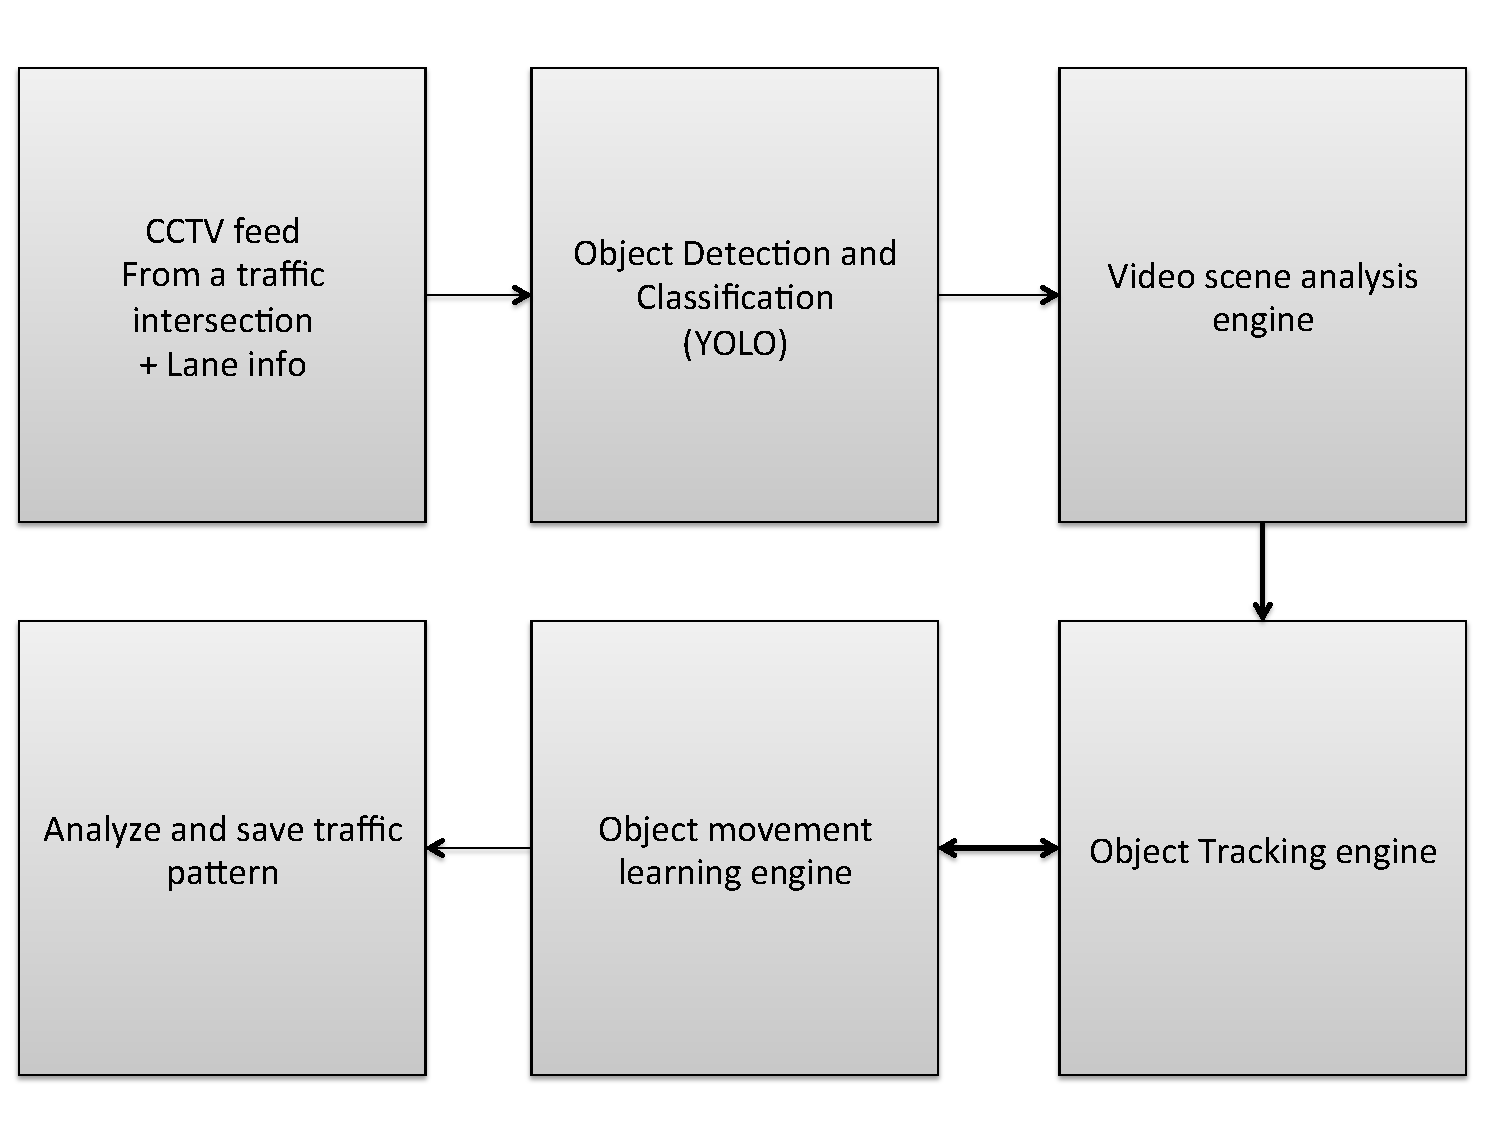
\includegraphics[scale=0.25]{fig/SystemArchitecture.pdf} %, width=\figwidthb
\caption{System Architecture.} \label{fig.sysarch}
\end{figure}
\subsubsection{CCTV feed and lane mapping}
We used OpenCV API's to feed in the data. 
Using these APIs we can read from a camera as well as from a file.
We mark the lanes on the field of view one time manually, such as in the figure \ref{fig.lanes_info} which has polygonal information of twelve lanes at a traffic intersection.
As seen in the figure, we grouped together multiple lanes into single lane as our traffic surveillance model was fine-tuned to get appropriate traffic flux over specific routes at this intersection. 
Each route is a pair of lanes.
\begin{figure}[!htbp]
\centering
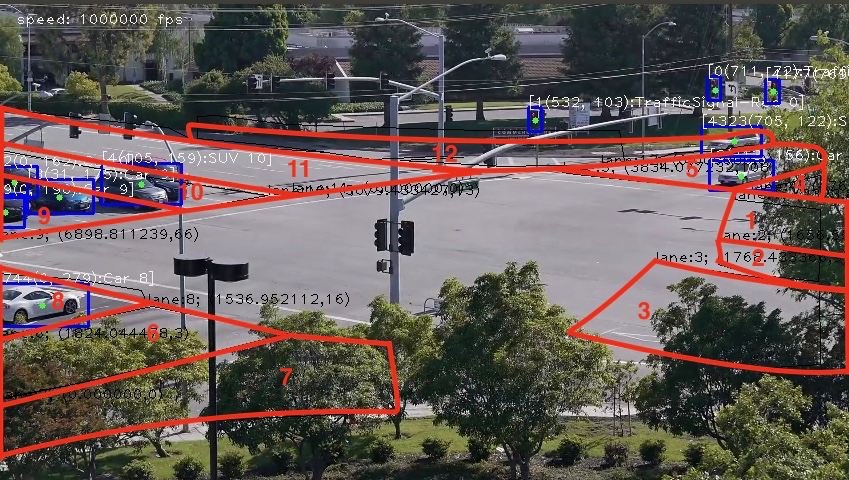
\includegraphics[scale=0.25]{fig/12_lane_info.png} %, width=\figwidthb
\caption{Polygonal lane information. As seen, this intersection has {12} marked lanes. Lane 1 to lane 11 is a route.} \label{fig.lanes_info}
\end{figure}

\subsubsection{Object detection and classification module}
We needed a real-time object detection model that shall give precise results.
Major models under consideration, after filtering by factors were Faster-RCNN \cite{Faster-RCNN} and YOLO \cite{YOLO_v1, YOLO_v2}.
When evaluated with pre-trained weights, we found that Faster-RCNN gave better precision than YOLOv2 \cite{YOLO_v2}. 
We generated ground truth for a video at an intersection.
We computed the Average Precision ({AP}) score as discussed in \cite{VOC_challenge}.
{AP} score for Faster-RCNN was evaluated at {0.83} and YOLOv2 at {0.71} for one particular classifier, namely car.
YOLO implements object detection and classification as a single regression problem \cite{YOLO_v1}.
It constructs the output bounding boxes directly from the input image pixels. 
Faster-RCNN on the other hand models a region proposal network \cite[p.~1]{Faster-RCNN} for detection.
The bounding boxes detected are then classified and passed through a third step of post-processing. 
Post-processing involves rescoring bounding boxes and filtration of duplicate boxes.
For the same reason, YOLO is inherently faster than other models.
We got better performance with YOLO than Faster-RCNN on a local machine. 

\subsubsection{Video scene analysis engine}


\subsubsection{Multi-algorithmic object tracking engine}

\subsubsection{Object movement learning engine}

\subsubsection{Analyze and save traffic pattern}


Math symbol: $\hat{r}_{n,m}^{(k)}$.

Equations:
\begin{align}
\mathbf{f}_t^n=\mathbf{R}_b^n \mathbf{f}_t^b + \mathbf{e}^n
\end{align}
where $\mathbf{e}^n$ is the error of the force that applied to the smartphone. The figure is shown in \figref{fig.doublefigure} and \figref{fig.structure}.

%\begin{figure}[htb]
%\centerline{\subfloat[Figure 1]{\includegraphics[width
%=0.5\linewidth]{fig/city.pdf} \label{fig.figure1}} \hfil
%\subfloat[Figure 2]{\includegraphics[width=0.5\linewidth]{fig/city.pdf}
%\label{fig.figure2}}
%} \caption{The figure for: (a) Figure1; (b) Figure2.} \label{fig.doublefigure}
%\end{figure}






\section{Related Work}\label{sec.related}
\cite{kumar2014accurate,Estimote}



\section{Conclusion}\label{sec.conclusion}


% conference papers do not normally have an appendix


% use section* for acknowledgment
%\section*{Acknowledgment}


%The authors would like to thank...





% trigger a \newpage just before the given reference
% number - used to balance the columns on the last page
% adjust value as needed - may need to be readjusted if
% the document is modified later
%\IEEEtriggeratref{8}
% The "triggered" command can be changed if desired:
%\IEEEtriggercmd{\enlargethispage{-5in}}

% references section

% can use a bibliography generated by BibTeX as a .bbl file
% BibTeX documentation can be easily obtained at:
% http://mirror.ctan.org/biblio/bibtex/contrib/doc/
% The IEEEtran BibTeX style support page is at:
% http://www.michaelshell.org/tex/ieeetran/bibtex/
%\bibliographystyle{IEEEtran}
% argument is your BibTeX string definitions and bibliography database(s)
%\bibliography{IEEEabrv,../bib/paper}
%
% <OR> manually copy in the resultant .bbl file
% set second argument of \begin to the number of references
% (used to reserve space for the reference number labels box)

%\bibliographystyle{IEEEtran}
%\bibliography{IEEEmybib}
\begin{thebibliography}{1}
%
%\bibitem{IEEEhowto:kopka}
%H.~Kopka and P.~W. Daly, \emph{A Guide to \LaTeX}, 3rd~ed.\hskip 1em plus
%  0.5em minus 0.4em\relax Harlow, England: Addison-Wesley, 1999.
%

\bibitem{YOLO_v1}
J. Redmon et al. (2016, May 9). 
\textit{You only look once: unified, real-time object detection (5th ed.)} [Online]. Available: https://arxiv.org/abs/1506.02640

\bibitem{YOLO_v2}
J. Redmon and A. Farhadi. (2016, December 25). 
\textit{YOLO9000: Better, Faster, Stronger} [Online]. Available: https://arxiv.org/abs/1612.08242

\bibitem{darknet}
J. Redmon. (2013?2016) 
\textit{Darknet: Open source neural networks in c} [Online]. Available: http://pjreddie.com/darknet/

\bibitem{Faster-RCNN}
S. Ren et al. (2016, January 6). 
\textit{Faster R-CNN: towards real-time object detection with region proposal networks} [Online]. Available: https://arxiv.org/abs/1506.01497


\bibitem{VOC_challenge}
M. Everingham et al., "The Pascal Visual Object Classes (VOC) Challenge,"
\textit{International Journal of Computer Vision.}, vol. 88, no. 2, pp. 303-338, June 2010.


\end{thebibliography}




% that's all folks
\end{document}


